% Rozdział aktywny po restrukturyzacji DT.
\section{Średnie Fouriera, jądro Fejéra i tożsamość Parsevala}
\providecommand{\atlasref}[2]{#2}

\subsection{Dodatnie aproksymacje jedności na okręgu}

Niech $\mathrm dm(t)=(2\pi)^{-1}\mathrm d\lambda_1(t)$
oznacza unormowaną miarę Haara na $\mathbb T$.
Splot okresowy z funkcją $K\in L^1(\mathbb T)$
zapisujemy jako
\[
 (K*f)(x)=\int_{\mathbb T}K(t)f(x-t)\,\mathrm dm(t).
\]
Dla $f\in L^1$ całka istnieje prawie wszędzie:
z twierdzenia Tonellego i niezmienniczości miary
względem przesunięć całka podwójna z modułu
jest równa $\|K\|_1\|f\|_1$.
Jeżeli $K$ i $f$ są ciągłe, całka istnieje
w każdym punkcie i określa funkcję ciągłą
przez jednostajną ciągłość $f$.

\begin{definicja}[Dodatnia aproksymacja jedności]
\label{def:dt-periodic-approximate-identity}
Rodzinę $(K_\nu)$ nieujemnych funkcji z
$L^1(\mathbb T)$ nazywamy dodatnią aproksymacją
jedności, jeśli $\int_{\mathbb T} K_\nu\,\mathrm dm=1$
oraz dla każdego $0<\delta<\pi$ zachodzi
\[
 \int_{\delta\le |t|\le\pi}K_\nu(t)\,\mathrm dm(t)
 \longrightarrow0.
\]
Parametr $\nu$ może na przykład dążyć do
nieskończoności albo do brzegu przedziału parametrów.
\end{definicja}

\begin{twierdzenie}[Aproksymacja jednostajna i w normie $L^p$]
\label{thm:dt-periodic-approximate-identity}
Jeśli $(K_\nu)$ jest dodatnią aproksymacją jedności,
to $K_\nu*f\to f$ jednostajnie dla $f\in C(\mathbb T)$,
a dla $f\in L^p(\mathbb T)$, $1\le p<\infty$,
zbieżność zachodzi w normie $L^p$.
Ponadto $\|K_\nu*f\|_p\le\|f\|_p$
dla $1\le p\le\infty$.
\end{twierdzenie}
\begin{proof}
Dla skończonego $p$ nierówność Jensena względem
miary probabilistycznej $K_\nu\,\mathrm dm$ daje
\[
 |(K_\nu*f)(x)|^p
 \le\int_{\mathbb T}K_\nu(t)|f(x-t)|^p\,\mathrm dm(t).
\]
Całkując i stosując twierdzenie Tonellego oraz
niezmienniczość miary, otrzymujemy kontraktywność.
Dla $p=\infty$ wynika ona wprost z ograniczenia
modułu funkcji przez jej kres istotny.
Dla $f$ ciągłej, po odjęciu $f(x)$ pod całką,
jednostajna ciągłość daje dla dowolnego
$\varepsilon>0$ takie $\delta>0$, że
\[
 \|K_\nu*f-f\|_\infty
 \le\varepsilon+2\|f\|_\infty
 \int_{\delta\le|t|\le\pi}K_\nu(t)\,\mathrm dm(t).
\]
Drugi składnik dąży do zera.

Dla $1\le p<\infty$ funkcje ciągłe okresowe
są gęste w $L^p(\mathbb T)$: przedłużamy funkcję
z $(-\pi,\pi)$ przez zero na $\R$, najpierw obcinamy
ją do $[-\pi+\eta,\pi-\eta]$ (błąd dąży do zera
przez zbieżność zmajoryzowaną), a następnie
aproksymujemy przez funkcję testową z
Twierdzenia~\ref{thm:dt-test-density}.
Mnożąc tę funkcję przez gładkie odcięcie
o wartościach w $[0,1]$, równe $1$ na obciętym
przedziale i o nośniku w $(-\pi,\pi)$
(Lemat~\ref{lem:cutoffs17}), nie zwiększamy błędu
względem funkcji obciętej. Okresowe przedłużenie
wyniku jest ciągłe. Wybieramy więc $g\in C(\mathbb T)$
z $\|f-g\|_p<\varepsilon$.
Z kontraktywności i jednostajnej zbieżności dla $g$
wynika
\[
 \|K_\nu*f-f\|_p
 \le 2\varepsilon+\|K_\nu*g-g\|_\infty.
\]
Dowolność $\varepsilon$ kończy dowód.
\end{proof}

\subsection{Jądro Fejéra i średnie Cesàra}

\begin{lemat}[Jądro Fejéra]
\label{lem:dt-series-fejer}
Dla całkowitego $N\geq0$ niech
\begin{equation}\label{eq:dt-series-fejer}
 F_N(t)=\frac1{N+1}\left|\sum_{j=0}^Ne^{ijt}\right|^2
 =\frac1{N+1}\left(\frac{\sin((N+1)t/2)}{\sin(t/2)}\right)^2
\end{equation}
(w punktach $t\in2\pi\mathbb Z$ przyjmujemy
$F_N(t)=N+1$, zgodnie z pierwszą postacią wzoru). Wówczas $F_N\ge0$,
$(2\pi)^{-1}\int_{-\pi}^{\pi}F_N(t)\,\mathrm d\lambda_1(t)=1$ oraz
dla każdego $\delta\in(0,\pi)$
$\int_{\delta\le|t|\le\pi}F_N(t)\,\mathrm d\lambda_1(t)\to0$.
\end{lemat}
\begin{proof}
Nieujemność jest bezpośrednia z definicji.
Dla $t\notin2\pi\mathbb Z$ z sumy geometrycznej
$\sum_{j=0}^N e^{ijt}=(1-e^{i(N+1)t})/(1-e^{it})$
i tożsamości $|1-e^{i\alpha}|=2|\sin(\alpha/2)|$
otrzymujemy drugą postać~\eqref{eq:dt-series-fejer}.
Rozwijając kwadrat modułu, mamy
\[
 F_N(t)=\frac1{N+1}\sum_{j,\ell=0}^N e^{i(j-\ell)t}
 =\sum_{|k|\leq N}\left(1-\frac{|k|}{N+1}\right)e^{ikt}.
\]
Dla ustalonego $|k|\leq N$ istnieje dokładnie
$N+1-|k|$ par $(j,\ell)$ z różnicą $j-\ell=k$:
dla $k\geq0$ wybieramy $\ell=0,\ldots,N-k$,
a dla $k<0$ zamieniamy role indeksów.
Wyraz stały jest równy $1$, a pozostałe
wykładniki mają całkę zero na pełnym okresie,
skąd normalizacja. Gdy $\delta\leq|t|\leq\pi$,
mamy $|\sin(t/2)|\geq\sin(\delta/2)>0$.
Dlatego
\[
 \int_{\delta\leq|t|\leq\pi}F_N(t)\,\mathrm d\lambda_1(t)
 \leq\frac{2\pi}{(N+1)\sin^2(\delta/2)}
 \longrightarrow0.
\]
\end{proof}

\begin{twierdzenie}[Fejér i zupełność układu trygonometrycznego]
\label{thm:dt-series-fejer}
Niech $f\in C(\mathbb T)$. Średnie Cesàra
$\sigma_N f=(N+1)^{-1}\sum_{j=0}^N S_jf$
zbieżne są jednostajnie do $f$ na $\mathbb T$.
W konsekwencji wielomiany trygonometryczne są gęste
w $C(\mathbb T)$ w normie supremum i w $L^2(\mathbb T)$
w normie $L^2$.
\end{twierdzenie}
\begin{proof}
W średniej z sum częściowych współczynnik
przy $\widehat f(k)e^{ikx}$ wynosi
$(N+1-|k|)/(N+1)$ dla $|k|\leq N$, ponieważ
wyraz ten występuje dla $j=|k|,\ldots,N$.
Z drugiej strony podstawienie $y=x-t$ daje
\[
 \frac1{2\pi}\int_{-\pi}^{\pi}e^{ikt}f(x-t)\,
 \mathrm d\lambda_1(t)=e^{ikx}\widehat f(k).
\]
Po podstawieniu całkujemy po odcinku
$[x-\pi,x+\pi]$, który możemy zastąpić
$[-\pi,\pi]$, gdyż $f(y)e^{-iky}$ jest
$2\pi$-okresowa i całka po pełnym okresie
nie zależy od jego początku (przez podział
odcinka i przesunięcie o wielokrotność okresu).
Rozwinięcie skończone z lematu~\ref{lem:dt-series-fejer}
daje więc
\[
 \sigma_Nf(x)=\frac1{2\pi}\int_{-\pi}^{\pi}
 F_N(t)f(x-t)\,\mathrm d\lambda_1(t).
\]
Z Lematu~\ref{lem:dt-series-fejer} wynika, że
$(F_N)$ jest dodatnią aproksymacją jedności.
Stąd Twierdzenie~\ref{thm:dt-periodic-approximate-identity}
daje jednostajną zbieżność dla funkcji ciągłych
oraz zbieżność w normie $L^2$ dla funkcji z $L^2$:
tożsamość splotowa obowiązuje także dla $f\in L^1$,
ponieważ użyto jedynie skończonych sum i całek.
Każda $\sigma_Nf$ jest wielomianem trygonometrycznym,
co dowodzi obu twierdzeń o gęstości.
\end{proof}

\begin{wniosek}[Średnie Fejéra w przestrzeniach $L^p$]
\label{cor:dt-fejer-lp}
Dla każdego $1\le p<\infty$ i $f\in L^p(\mathbb T)$
średnie $\sigma_Nf$ zbiegają do $f$ w normie $L^p$.
Wielomiany trygonometryczne są zatem gęste
w każdej z tych przestrzeni.
\end{wniosek}
\begin{proof}
Lemat~\ref{lem:dt-series-fejer} pokazuje, że
$(F_N)$ jest dodatnią aproksymacją jedności.
Tożsamość $\sigma_N f=F_N*f$ z dowodu
Twierdzenia~\ref{thm:dt-series-fejer} obowiązuje
również dla $f\in L^1$, ponieważ wymaga jedynie
zamiany skończonej sumy z całką.
Stosujemy Twierdzenie~\ref{thm:dt-periodic-approximate-identity}.
Każda średnia $\sigma_Nf$ jest wielomianem trygonometrycznym.
\end{proof}

\subsection{Zupełność układu i tożsamość Parsevala}

\begin{twierdzenie}[Zbieżność w $L^2$ i tożsamość Parsevala]
\label{thm:dt-series-parseval}
Dla dowolnego $f\in L^2(\mathbb T)$ zachodzą
$S_Nf\to f$ w normie $L^2$ oraz
\begin{equation}\label{eq:dt-series-parseval}
 \frac1{2\pi}\int_{-\pi}^{\pi}|f(x)|^2\,\mathrm d\lambda_1(x)
 =\sum_{k\in\mathbb Z}|\widehat f(k)|^2.
\end{equation}
\end{twierdzenie}
\begin{proof}
Dla $\varepsilon>0$ wybieramy wielomian trygonometryczny $p$
z $\|f-p\|_2<\varepsilon$. Dla $N$ nie mniejszych niż stopień
$p$ mamy $S_Np=p$. Ponieważ $f-S_Nf$ jest
prostopadła do przestrzeni, do której należy
$S_Nf-p$, zachodzi
\[
 \|f-p\|_2^2=\|f-S_Nf\|_2^2+\|S_Nf-p\|_2^2.
\]
Zatem $\|f-S_Nf\|_2\leq\|f-p\|_2<\varepsilon$,
co dowodzi zbieżności.
W konsekwencji $\|S_Nf\|_2\to\|f\|_2$,
a z tożsamości $\|S_Nf\|_2^2=
\sum_{|k|\leq N}|\widehat f(k)|^2$
w lemacie~\ref{lem:dt-series-bessel} otrzymujemy
\eqref{eq:dt-series-parseval}, ponieważ sumy
nieujemnych wyrazów rosną do pełnej sumy po $\mathbb Z$.
\end{proof}

\begin{uwaga}[Jakiego rodzaju zbieżność została udowodniona?]
Sama zbieżność w normie $L^2$ nie pociąga
za sobą zbieżności jednostajnej ani punktowej
całego ciągu. Nie rozstrzygamy tutaj odrębnego
zagadnienia zbieżności prawie wszędzie sum
częściowych Fouriera. Dla funkcji ciągłych jednostajnie zbieżne są
\emph{średnie Fejéra}, niekoniecznie zwykłe sumy $S_N$.
Dla gładkich funkcji zachodzi dodatkowe szybkie zanikanie
współczynników, co wykażemy w następnym rozdziale.
\end{uwaga}

\subsection{Jądro Poissona i sumowanie Abela}

\begin{twierdzenie}[Jądro Poissona na okręgu]
\label{thm:dt-periodic-poisson}
Dla $0\le r<1$ kładziemy
\[
 P_r(t)=\frac{1-r^2}{1-2r\cos t+r^2}.
\]
Wówczas
\[
 P_r(t)=\sum_{k\in\mathbb Z}r^{|k|}e^{ikt}
 =1+2\sum_{k=1}^\infty r^k\cos(kt),
\]
przy czym wyraz dla $k=0$ wynosi $1$ także
dla $r=0$. Szereg jest bezwzględnie i jednostajnie
zbieżny dla każdego ustalonego $r<1$.
Rodzina $(P_r)$ jest dodatnią aproksymacją jedności
przy $r\uparrow1$.
\end{twierdzenie}
\begin{proof}
Z sumy szeregu geometrycznego i jego sprzężenia
zespolonego otrzymujemy
\[
 1+\frac{re^{it}}{1-re^{it}}
   +\frac{re^{-it}}{1-re^{-it}}
 =\frac{1-r^2}{|1-re^{it}|^2}.
\]
Jednostajna zbieżność wynika z majoranty
$\sum_{k\ge1}2r^k$. Nieujemność wynika
z ilorazu, a całkowanie wyraz po wyrazie
i ortogonalność dają $\int_{\mathbb T}P_r\,\mathrm dm=1$.
Dla $\delta\le|t|\le\pi$ i $r\ge1/2$ mamy
\[
 |1-re^{it}|^2=(1-r)^2+2r(1-\cos t)
 \ge1-\cos\delta>0.
\]
Stąd całka poza otoczeniem zera jest ograniczona
przez $(1-r^2)/(1-\cos\delta)$ i dąży do zera.
\end{proof}

\begin{wniosek}[Sumowanie Abela szeregów Fouriera]
\label{cor:dt-poisson-abel}
Dla $f\in L^1(\mathbb T)$ i $0\le r<1$ zachodzi
\[
 (P_r*f)(x)=\sum_{k\in\mathbb Z}r^{|k|}
 \widehat f(k)e^{ikx}.
\]
Jeżeli $f\in C(\mathbb T)$, lewa strona zbiega
jednostajnie do $f$ przy $r\uparrow1$.
Jeżeli $f\in L^p$, $1\le p<\infty$,
zbieżność zachodzi w normie $L^p$.
\end{wniosek}
\begin{proof}
Jednostajna zbieżność szeregu jądra i całkowalność
$f$ pozwalają zamienić szereg z całką splotową.
Podstawienie $y=x-t$ daje współczynniki Fouriera.
Ponadto $|\widehat f(k)|\le\|f\|_{L^1(\mathbb T)}$,
więc wynikowy szereg jest bezwzględnie i jednostajnie
zbieżny względem $x$ dla ustalonego $r<1$.
Oba rodzaje zbieżności wynikają z
Twierdzenia~\ref{thm:dt-periodic-poisson}
i Twierdzenia~\ref{thm:dt-periodic-approximate-identity}.
\end{proof}

Jądra Fejéra i Poissona mają masę $1$ i są nieujemne,
w odróżnieniu od jądra Dirichleta. Dzięki temu
średnie Cesàra i sumy Abela odzyskują każdą
funkcję ciągłą jednostajnie, mimo że zwykłe
sumy częściowe nie mają takiej własności
(Wniosek~\ref{cor:dt-dirichlet-unbounded}).

\begin{center}
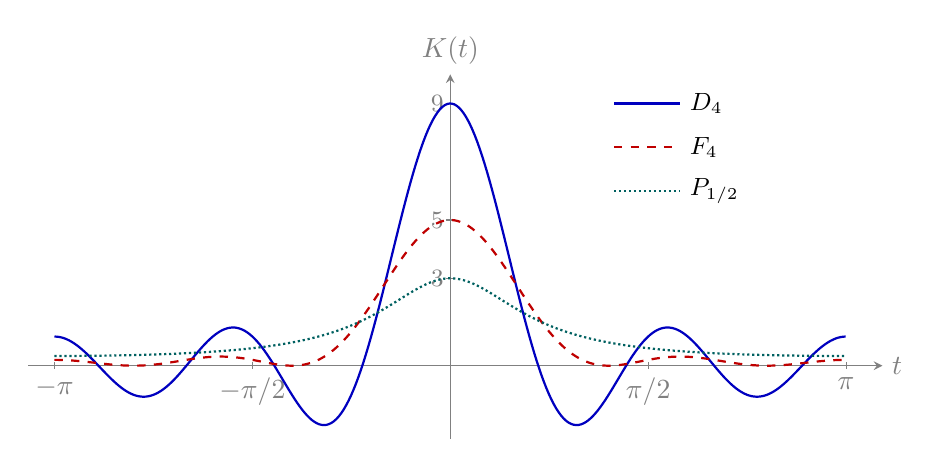
\begin{tikzpicture}[x=1.6cm,y=0.37cm,>=stealth]
 \draw[->,gray] (-3.35,0)--(3.43,0) node[right] {$t$};
 \draw[->,gray] (0,-2.5)--(0,10) node[above] {$K(t)$};
 \foreach \x/\lab in {-3.14159/{-\pi},-1.5708/{-\pi/2},1.5708/{\pi/2},3.14159/{\pi}}
   {\draw[gray] (\x,0.12)--(\x,-0.12) node[below=2pt,fill=white,inner sep=1pt] {$\lab$};}
 \foreach \y in {3,5,9}
   {\draw[gray] (-0.04,\y)--(0.04,\y) node[left=3pt,fill=white,inner sep=1pt] {\small $\y$};}
 \draw[blue!75!black,thick,domain=-3.14159:3.14159,samples=321,variable=\x]
 plot ({\x},{1+2*cos(deg(\x))+2*cos(deg(2*\x))+2*cos(deg(3*\x))+2*cos(deg(4*\x))});
 \draw[red!75!black,thick,dashed,domain=-3.14159:3.14159,samples=321,variable=\x]
 plot ({\x},{1+1.6*cos(deg(\x))+1.2*cos(deg(2*\x))+0.8*cos(deg(3*\x))+0.4*cos(deg(4*\x))});
 \draw[teal!75!black,thick,densely dotted,domain=-3.14159:3.14159,samples=321,variable=\x]
 plot ({\x},{0.75/(1.25-cos(deg(\x)))});
 \draw[blue!75!black,thick] (1.3,9)--(1.82,9) node[right,black] {\small $D_4$};
 \draw[red!75!black,thick,dashed] (1.3,7.5)--(1.82,7.5) node[right,black] {\small $F_4$};
 \draw[teal!75!black,thick,densely dotted] (1.3,6)--(1.82,6) node[right,black] {\small $P_{1/2}$};
\end{tikzpicture}

\small Porównanie trzech jąder na jednym okresie.
Wszystkie mają unormowaną całkę równą $1$,
ale tylko jądro Dirichleta przyjmuje wartości ujemne.
Wykresy korzystają z rozwinięć trygonometrycznych
i wzoru wymiernego na jądro Poissona.
\end{center}

\subsection{Iloczynowe aproksymacje jedności na torusie}

Na $\mathbb T^d$ piszemy
$\mathrm dm_d(t)=(2\pi)^{-d}\mathrm d\lambda_d(t)$
na kostce fundamentalnej $Q=[-\pi,\pi]^d$.
Splot definiujemy analogicznie jak w jednym wymiarze.
Otoczenia zera możemy opisywać przez
$\max_j|t_j|<\delta$, gdzie $0<\delta<\pi$.

\begin{twierdzenie}[Aproksymacje jedności na torusie]
\label{thm:dt-torus-approximate-identity}
Niech $K_\nu\ge0$ na $\mathbb T^d$,
$\int K_\nu\,\mathrm dm_d=1$ oraz
\[
 \int_{\max_j|t_j|\ge\delta} K_\nu(t)\,\mathrm dm_d(t)
 \longrightarrow0
 \qquad(0<\delta<\pi).
\]
Wówczas $K_\nu*f\to f$ jednostajnie dla
$f\in C(\mathbb T^d)$ i w normie $L^p$ dla
$f\in L^p(\mathbb T^d)$, $1\le p<\infty$.
Operator splotu jest kontrakcją na $L^p$
dla $1\le p\le\infty$.
\end{twierdzenie}
\begin{proof}
Dowód Twierdzenia~\ref{thm:dt-periodic-approximate-identity}
przenosi się na torus: nierówność Jensena,
twierdzenie Tonellego i niezmienniczość $m_d$
względem przesunięć dają
$\|K_\nu*f\|_p\le\|f\|_p$.
Dla $f$ ciągłej wybieramy $\delta$ tak,
aby $\max_j|t_j|<\delta$ implikowało
$|f(x-t)-f(x)|<\varepsilon$ dla wszystkich $x$.
Podział całki na to otoczenie i jego dopełnienie
daje oszacowanie
\[
 \|K_\nu*f-f\|_\infty
 \le\varepsilon+2\|f\|_\infty
 \int_{\max_j|t_j|\ge\delta}K_\nu(t)\,\mathrm dm_d(t).
\]
W konsekwencji zachodzi jednostajna zbieżność.

Uzasadnimy gęstość $C(\mathbb T^d)$ w $L^p$
dla skończonego $p$. Przedłużamy $f|_Q$ zerem
na $\R^d$ i obcinamy ją do kostki
$Q_\eta=[-\pi+\eta,\pi-\eta]^d$.
Błąd w normie $L^p$ dąży do zera przez
zbieżność zmajoryzowaną, gdyż brzeg $Q$
ma miarę Lebesgue'a zero.
Aproksymujemy obciętą funkcję przez
$g\in\mathcal D(\R^d)$ (Twierdzenie~\ref{thm:dt-test-density}).
Wybieramy $\chi\in\mathcal D((-\pi,\pi)^d)$
o wartościach w $[0,1]$ i równą $1$ na $Q_\eta$
(Lemat~\ref{lem:cutoffs17}).
Mnożenie $g$ przez $\chi$ nie zwiększa błędu
względem obciętej funkcji, ponieważ ta ostatnia
nie zmienia się przy mnożeniu przez $\chi$.
Przedłużenie okresowe $\chi g$ jest gładkie,
gdyż funkcja znika w otoczeniu brzegu $Q$.
W ten sposób otrzymujemy żądaną gęstość.
Kontraktywność i aproksymacja przez funkcje ciągłe
kończą dowód tak jak w jednym wymiarze.
\end{proof}

\begin{wniosek}[Jądra Fejéra i Poissona na torusie]
\label{cor:dt-torus-fejer-poisson}
Rodziny
\[
 F_N^{[d]}(t)=\prod_{j=1}^dF_N(t_j),\qquad
 P_r^{[d]}(t)=\prod_{j=1}^dP_r(t_j)
\]
są dodatnimi aproksymacjami jedności na $\mathbb T^d$
odpowiednio przy $N\to\infty$ i $r\uparrow1$.
Dla $f\in L^1(\mathbb T^d)$ zachodzą wzory
\[
 \begin{aligned}
 (F_N^{[d]}*f)(x)
 &=\sum_{\max_j|k_j|\le N}
 \widehat f(k)e^{ik\cdot x}
 \prod_{j=1}^d\left(1-\frac{|k_j|}{N+1}\right),\\
 (P_r^{[d]}*f)(x)
 &=\sum_{k\in\mathbb Z^d}r^{\sum_j|k_j|}
 \widehat f(k)e^{ik\cdot x}.
 \end{aligned}
\]
W szczególności wielomiany trygonometryczne są
gęste w $C(\mathbb T^d)$ oraz w $L^p(\mathbb T^d)$
dla $1\le p<\infty$.
\end{wniosek}
\begin{proof}
Niech $H$ oznacza jedno z jąder jednowymiarowych.
Twierdzenie Fubiniego daje
$\int_{\mathbb T^d}\prod_j H(t_j)\,\mathrm dm_d=1$.
Zbiór $\{\max_j|t_j|\ge\delta\}$ jest sumą
zbiorów $\{|t_j|\ge\delta\}$, więc z nieujemności
oraz normalizacji $H$ dostajemy
\[
 \int_{\max_j|t_j|\ge\delta}\prod_j H(t_j)\,\mathrm dm_d
 \le d\int_{|t|\ge\delta}H(t)\,\mathrm dm(t).
\]
Prawa strona dąży do zera na mocy
Lematu~\ref{lem:dt-series-fejer} albo
Twierdzenia~\ref{thm:dt-periodic-poisson}.
Wstawiając rozwinięcia jednowymiarowych jąder
i mnożąc je, otrzymujemy podane szeregi splotowe.
W przypadku Poissona uzasadnienie zamiany szeregu
z całką wynika z bezwzględnej i jednostajnej zbieżności:
\[
 \sum_{k\in\mathbb Z^d} r^{\sum_j|k_j|}
 =\left(1+2\sum_{n\ge1}r^n\right)^d
 =\left(\frac{1+r}{1-r}\right)^d<\infty.
\]
Dla $r=0$ współczynnik przy $k=0$ wynosi $1$.
Twierdzenie~\ref{thm:dt-torus-approximate-identity}
daje zbieżność splotów, a sploty z jądrem Fejéra
są wielomianami trygonometrycznymi.
\end{proof}

\subsection{Twierdzenie Riesza--Fischera i unitarność}

\begin{twierdzenie}[Parseval i Riesz--Fischer na torusie]
\label{thm:dt-torus-riesz-fischer}
Układ $(e^{ik\cdot x})_{k\in\mathbb Z^d}$
jest bazą ortonormalną przestrzeni Hilberta
$L^2(\mathbb T^d,m_d)$.
Odwzorowanie
\[
 \mathcal F_{\mathbb T^d}: L^2(\mathbb T^d,m_d)
 \longrightarrow\ell^2(\mathbb Z^d),\qquad
 f\longmapsto(\widehat f(k))_{k\in\mathbb Z^d}
\]
jest izomorfizmem unitarnym. W szczególności
dla $f,g\in L^2(\mathbb T^d)$ mamy
\[
 \langle f,g\rangle=
 \sum_{k\in\mathbb Z^d}\widehat f(k)
 \overline{\widehat g(k)}.
\]
Każdy ciąg $(c_k)\in\ell^2(\mathbb Z^d)$
jest ciągiem współczynników Fouriera dokładnie
jednego elementu $L^2(\mathbb T^d)$, a odwrotne
odwzorowanie jest dane szeregiem
\[
 f=\sum_{k\in\mathbb Z^d}c_ke^{ik\cdot x}
\]
zbieżnym bezwarunkowo w normie $L^2$.
\end{twierdzenie}
\begin{proof}
Ortonormalność wynika ze
Stwierdzenia~\ref{prop:dt-series-torus},
a zupełność z gęstości wielomianów trygonometrycznych
we Wniosku~\ref{cor:dt-torus-fejer-poisson}.
Niech $A_N=\{-N,\ldots,N\}^d$.
Rzut $S_{A_N}f$ jest najlepszym przybliżeniem
$f$ w rozpiętości odpowiednich harmonicznych:
dla wielomianu $p$ o indeksach w $A_N$
rozkład $f-p=(f-S_{A_N}f)+(S_{A_N}f-p)$
jest ortogonalny. Gęstość wielomianów daje
$S_{A_N}f\to f$ w $L^2$. Przechodząc do granicy
w tożsamości norm ze
Stwierdzenia~\ref{prop:dt-series-torus},
otrzymujemy
\[
 \|f\|_2^2=\sum_{k\in\mathbb Z^d}|\widehat f(k)|^2.
\]
To daje izometryczność i różnowartościowość.
Tożsamość iloczynów skalarnych wynika przez
przejście do granicy w
$\langle S_{A_N}f,S_{A_N}g\rangle$;
szereg iloczynów współczynników jest bezwzględnie
zbieżny z nierówności Cauchy'ego--Schwarza.

Dla dowolnego $(c_k)\in\ell^2$ kładziemy
$p_N=\sum_{k\in A_N}c_ke^{ik\cdot x}$.
Z ortonormalności dla $M>N$ mamy
\[
 \|p_M-p_N\|_2^2=\sum_{k\in A_M\setminus A_N}|c_k|^2
 \longrightarrow0
\]
jednostajnie względem $M>N$ przy $N\to\infty$,
ponieważ ogon szeregu kwadratów dąży do zera.
Z zupełności przestrzeni Hilberta istnieje
$f\in L^2$ takie, że $p_N\to f$ w normie.
Dla ustalonego $k$ funkcjonał
$f\mapsto\langle f,e^{ik\cdot x}\rangle$ jest ciągły
z nierówności Cauchy'ego--Schwarza, więc
$\widehat f(k)=c_k$. Dowodzi to surjektywności.
Jeżeli $A$ jest dowolnym skończonym zbiorem
zawierającym $A_N$, to udowodniona tożsamość norm
daje
\[
 \left\|f-\sum_{k\in A}c_ke^{ik\cdot x}\right\|_2^2
 =\sum_{k\notin A}|c_k|^2
 \le\sum_{k\notin A_N}|c_k|^2.
\]
Stąd wynika bezwarunkowa zbieżność (granica
po skończonych zbiorach skierowanych przez inkluzję),
a w szczególności niezależność od enumeracji indeksów.
\end{proof}

\subsection{Jednoznaczność i zastosowania tożsamości Parsevala}

\begin{wniosek}[Jednoznaczność współczynników Fouriera w $L^1$]
\label{cor:dt-fourier-l1-uniqueness}
Jeżeli $f,g\in L^1(\mathbb T^d)$ i
$\widehat f(k)=\widehat g(k)$ dla wszystkich
$k\in\mathbb Z^d$, to $f=g$ prawie wszędzie.
Jeżeli obie funkcje są ciągłe, równość zachodzi
w każdym punkcie.
\end{wniosek}
\begin{proof}
Dla $h=f-g$ wszystkie współczynniki znikają.
Wzór z Wniosku~\ref{cor:dt-torus-fejer-poisson}
daje $F_N^{[d]}*h=0$ dla każdego $N$.
Z Twierdzenia~\ref{thm:dt-torus-approximate-identity}
wynika $F_N^{[d]}*h\to h$ w $L^1$, a więc
$\|h\|_1=0$. Dla funkcji ciągłych niezerowa
wartość w jednym punkcie pociągałaby
niezerowość na otwartym zbiorze dodatniej miary.
\end{proof}

\begin{wniosek}[Odtwarzanie funkcji z bezwzględnie sumowalnych współczynników]
\label{cor:dt-fourier-l1-absolute}
Niech $f\in L^1(\mathbb T^d)$ i niech
$\sum_{k\in\mathbb Z^d}|\widehat f(k)|<\infty$.
Wówczas szereg
\[
 g(x)=\sum_{k\in\mathbb Z^d}\widehat f(k)e^{ik\cdot x}
\]
zbiega bezwzględnie i jednostajnie, a jego suma
jest ciągłym reprezentantem $f$.
Jeżeli $f$ jest ciągła, to $g=f$ punktowo.
\end{wniosek}
\begin{proof}
Kryterium Weierstrassa daje jednostajną
zbieżność, niezależną od enumeracji indeksów.
Całkowanie wyraz po wyrazie jest uzasadnione
jednostajną zbieżnością i skończonością miary.
Ortonormalność ze Stwierdzenia~\ref{prop:dt-series-torus}
daje $\widehat g(k)=\widehat f(k)$.
Stosujemy Wniosek~\ref{cor:dt-fourier-l1-uniqueness}.
\end{proof}

\begin{przyklad}[Sumy odwrotności kwadratów i czwartych potęg]
\label{ex:dt-parseval-zeta}
Dla okresowego przedłużenia $f(x)=x$ z
Przykładu~\ref{ex:dt-series-sawtooth}
mamy $\widehat f(0)=0$ oraz
$|\widehat f(n)|=1/|n|$ dla $n\ne0$,
na podstawie Stwierdzenia~\ref{prop:dt-series-real}.
Tożsamość Parsevala daje
\[
 \frac{\pi^2}{3}
 =\frac1{2\pi}\int_{-\pi}^{\pi}x^2\,\mathrm d\lambda_1(x)
 =2\sum_{n=1}^{\infty}\frac1{n^2}.
\]
Stąd $\sum_{n=1}^{\infty}n^{-2}=\pi^2/6$.

Dla $g(x)=x^2$ z Przykładu~\ref{ex:dt-series-quadratic}
mamy $\widehat g(0)=\pi^2/3$ oraz
$\widehat g(n)=2(-1)^n/n^2$ dla $n\ne0$.
Ze Wniosku~\ref{cor:dt-fourier-l1-absolute}
wynika tożsamość punktowa
\[
 x^2=\frac{\pi^2}{3}+4\sum_{n=1}^\infty
 \frac{(-1)^n}{n^2}\cos(nx),\qquad -\pi\le x\le\pi.
\]
Tożsamość Parsevala zastosowana do $g$ daje
\[
 \frac{\pi^4}{5}
 =\frac1{2\pi}\int_{-\pi}^{\pi}x^4\,\mathrm d\lambda_1(x)
 =\frac{\pi^4}{9}+8\sum_{n=1}^{\infty}\frac1{n^4}.
\]
Po odjęciu wyrazu stałego otrzymujemy
$\sum_{n=1}^{\infty}n^{-4}=\pi^4/90$.
\end{przyklad}

\subsection{Półgrupa Poissona}

\begin{twierdzenie}[Własność półgrupowa jąder Poissona]
\label{thm:dt-poisson-semigroup}
Niech $0\le r,s<1$. Na $\mathbb T^d$ zachodzi
$P_r^{[d]}*P_s^{[d]}=P_{rs}^{[d]}$.
Dla $t>0$ oznaczmy przez $Q_t$ operator splotu
z $P_{e^{-t}}^{[d]}$ i połóżmy $Q_0=I$.
Wówczas $(Q_t)_{t\ge0}$ jest półgrupą kontrakcji,
silnie ciągłą na $L^p(\mathbb T^d)$ dla
$1\le p<\infty$ oraz na $C(\mathbb T^d)$
z normą supremum.
\end{twierdzenie}
\begin{proof}
Dla $f,g\in L^1(\mathbb T^d)$ twierdzenie
Fubiniego i podstawienie $y=x-t$ dają
\[
 \widehat{f*g}(k)=\widehat f(k)\widehat g(k).
\]
Zastosowanie twierdzenia Fubiniego jest
uzasadnione całkowalnością modułu:
$\int\!\int |f(t)g(x-t)|\,\mathrm dm_d(x)\,\mathrm dm_d(t)
=\|f\|_1\|g\|_1$.
Z rozwinięcia jąder Poissona we
Wniosku~\ref{cor:dt-torus-fejer-poisson} wynika
$\widehat P_r^{[d]}(k)=r^{\sum_j|k_j|}$,
z konwencją $r^0=1$ także dla $r=0$.
Stąd współczynniki splotu są współczynnikami
$P_{rs}^{[d]}$. Jednoznaczność w $L^1$ i ciągłość
obu stron dają równość punktową.
Łączność splotu wynika z twierdzenia Fubiniego
dla trzech funkcji całkowalnych, a zatem
$Q_tQ_u=Q_{t+u}$; przypadek zerowego parametru
wynika z definicji $Q_0$.

Kontraktywność i silna ciągłość w zerze
wynikają z Twierdzenia~\ref{thm:dt-torus-approximate-identity}.
Dla $t\ge u\ge0$ i dla każdej rozważanej normy mamy
\[
 \|Q_tf-Q_uf\|
 =\|Q_u(Q_{t-u}f-f)\|
 \le\|Q_{t-u}f-f\|.
\]
To daje ciągłość przy każdym $t\ge0$.
\end{proof}

\begin{uwaga}
Dla $d>1$ jest to półgrupa odpowiadająca mnożnikowi
$\exp(-t\sum_j|k_j|)$, a nie mnożnikowi
$\exp(-t|k|)$ z normą euklidesową.
Obie konstrukcje zgadzają się w jednym wymiarze,
ale w wyższych wymiarach wyznaczają różne operatory.
\end{uwaga}

\begin{twierdzenie}[Generator półgrupy iloczynowej Poissona na $L^2$]
\label{thm:dt-poisson-generator-l2}
Niech $H=L^2(\mathbb T^d,m_d)$ i
$\rho(k)=\sum_{j=1}^d|k_j|$.
Generator $A$ półgrupy $(Q_t)$, określony
na zbiorze tych $f\in H$, dla których istnieje
granica w normie $H$
\[
 Af=\lim_{t\downarrow0}\frac{Q_tf-f}{t},
\]
ma dziedzinę
\[
 \operatorname{Dom}(A)=
 \left\{ f\in H:
 \sum_{k\in\mathbb Z^d}\rho(k)^2|\widehat f(k)|^2
 <\infty\right\},
 \qquad
 \widehat{Af}(k)=-\rho(k)\widehat f(k).
\]
Operator $A$ jest gęsto określony, domknięty,
samosprzężony i niedodatni, tj.
$\langle Af,f\rangle\le0$.
Dla $d=1$ jest to realizacja operatora
$-(-\partial_x^2)^{1/2}$ przez mnożniki Fouriera.
Dla $d>1$ odpowiada ona sumie operatorów
$-\sum_{j=1}^d(-\partial_{x_j}^2)^{1/2}$,
gdzie każdy pierwiastek oznacza mnożnik $|k_j|$
na właściwej dziedzinie w $L^2$.
\end{twierdzenie}
\begin{proof}
Na mocy Wniosku~\ref{cor:dt-torus-fejer-poisson}
i Twierdzenia~\ref{thm:dt-torus-riesz-fischer}
półgrupa na $H$ odpowiada mnożnikom
$e^{-t\rho(k)}$ na $\ell^2(\mathbb Z^d)$.
Ciągłość funkcjonału wyznaczającego współczynnik
Fouriera pokazuje, że jeżeli ilorazy różnicowe
zbiegają do $g\in H$, to dla każdego $k$
\[
 \widehat g(k)=
 \lim_{t\downarrow0}\frac{e^{-t\rho(k)}-1}{t}
 \widehat f(k)=-\rho(k)\widehat f(k).
\]
Z tożsamości Parsevala wynika konieczność
warunku sumowalności.

Odwrotnie, dla $f$ spełniającej ten warunek
twierdzenie Riesza--Fischera daje $g\in H$
o współczynnikach $-\rho(k)\widehat f(k)$.
Dla $u\ge0$ zachodzi $0\le1-e^{-u}\le u$
(z całkowania $e^{-v}\le1$ po $[0,u]$).
Wobec tego
\[
 \left|
 \left(\frac{e^{-t\rho(k)}-1}{t}+\rho(k)\right)
 \widehat f(k)\right|^2
 \le \rho(k)^2|\widehat f(k)|^2.
\]
Lewy składnik dąży do zera dla każdego $k$,
a prawa strona jest sumowalna.
Z twierdzenia o zbieżności zmajoryzowanej
dla miary liczącej i z Parsevala wynika
zbieżność ilorazów różnicowych do $g$ w $H$.

Dziedzina zawiera wielomiany trygonometryczne,
a więc jest gęsta. Unitarne odwzorowanie Fouriera
przenosi $A$ na mnożenie przez rzeczywisty ciąg
$-\rho$ na maksymalnej dziedzinie w $\ell^2$.
Domkniętość widać bezpośrednio: jeśli $c_n\to c$
oraz $-\rho c_n\to b$ w $\ell^2$, to zbieżność
każdej współrzędnej daje $b_k=-\rho(k)c_k$.
W szczególności $c$ należy do dziedziny.
Symetryczność wynika z rzeczywistości $\rho$.
Jeżeli $b$ należy do dziedziny operatora
sprzężonego i $h=A^*b$ w reprezentacji ciągowej,
to z definicji sprzężenia, testując na ciągu
jednostkowym w pozycji $k$, otrzymujemy
$h_k=-\rho(k)b_k$. Ponieważ $h\in\ell^2$,
wektor $b$ należy do dziedziny mnożenia.
Symetryczność daje inkluzję przeciwną,
a więc operator jest samosprzężony.
Ponadto z Parsevala
\[
 \langle Af,f\rangle
 =-\sum_{k\in\mathbb Z^d}\rho(k)|\widehat f(k)|^2
 \le0.
\]
Szereg jest bezwzględnie zbieżny z nierówności
Cauchy'ego--Schwarza.
Dla $d=1$ symbol $-\partial_x^2$ na wykładnikach
wynosi $k^2$, a jego nieujemny pierwiastek
w reprezentacji Fouriera ma symbol $|k|$.
Analogicznie dla każdej współrzędnej.
Dziedzina sumy jest przecięciem dziedzin tych
pierwiastków: $|k_j|\le\rho(k)$ oraz
$\rho(k)^2\le d\sum_j|k_j|^2$.
\end{proof}

\begin{wniosek}[Regularność półgrupy Poissona]
\label{cor:dt-poisson-smoothing}
Dla $f\in L^2(\mathbb T^d)$ i $t>0$
funkcja $Q_tf$ ma gładkiego reprezentanta.
Dla każdego $m\in\N_0$ istnieje stała $C_m$
taka, że
\[
 \|A^mQ_tf\|_2\le C_m t^{-m}\|f\|_2.
\]
Ponadto $u(t)=Q_tf$ jest różniczkowalna w normie
$L^2$ dla $t>0$, spełnia $u'(t)=Au(t)$
i $u(t)\to f$ w $L^2$ dla $t\downarrow0$.
\end{wniosek}
\begin{proof}
Dla ustalonego $t>0$ i wielowskaźnika $\alpha$
szereg
\[
 \sum_k(ik)^\alpha e^{-t\rho(k)}\widehat f(k)e^{ik\cdot x}
\]
jest jednostajnie i bezwzględnie zbieżny:
$|\widehat f(k)|\le\|f\|_2$,
$|k^\alpha|\le\rho(k)^{|\alpha|}$ dla $k\ne0$,
a $\rho(k)^{|\alpha|}e^{-t\rho(k)/2}$ jest ograniczone.
Sumowalność $\sum_k e^{-t\rho(k)/2}$ wynika
z iloczynu szeregów geometrycznych, jak w dowodzie
Wniosku~\ref{cor:dt-torus-fejer-poisson}.
Kryterium Weierstrassa i twierdzenie o różniczkowaniu
szeregu funkcji, stosowane kolejno do każdej zmiennej,
dają gładkość reprezentanta.
Iteracja opisu generatora pokazuje, że $Q_tf$
należy do dziedziny wszystkich jego potęg.
Z Parsevala oraz
$\sup_{v\ge0}v^me^{-v}<\infty$
(dla $m=0$ przyjmujemy $C_0=1$)
otrzymujemy żądane oszacowanie.
Różniczkowanie mnożnika $e^{-t\rho(k)}$
względem $t$ daje $-\rho(k)e^{-t\rho(k)}$.
Dla $|h|<t/2$ odpowiednie ilorazy różnicowe
są ograniczone przez $\rho(k)e^{-t\rho(k)/2}$,
z twierdzenia o wartości średniej.
Ten mnożnik jest ograniczony niezależnie od $k$,
więc zbieżność zmajoryzowana dla miary liczącej
i Parseval uzasadniają różniczkowanie w normie $L^2$.
Warunek początkowy wynika z silnej ciągłości półgrupy.
\end{proof}
